% \section{Resultados y evaluación}
%
% Se presenta una evaluación del rendimiento de tres variantes de RF-DETR (Nano, Small, Large) en comparación con HerdNet, el modelo de referencia establecido en la literatura para la detección de fauna en manadas densas. Los resultados se organizan en subsecciones que analizan: (1) el rendimiento cuantitativo general, (2) la precisión por especie y el impacto en clases minoritarias, (3) el efecto del HNM, y (4) la eficiencia computacional y viabilidad práctica de los modelos.

\section{Results and Evaluation}

An evaluation of the performance of three RF-DETR variants (Nano, Small, Large) is presented in comparison with HerdNet, the reference model established in the literature for wildlife detection in dense herds. The results are organized in subsections that analyze: (1) overall quantitative performance, (2) per-species accuracy and impact on minority classes, (3) the effect of HNM, and (4) computational efficiency and practical viability of the models.

% \subsection{Rendimiento Cuantitativo Comparativo}
%
% \subsubsection{Métricas}
%
% Para evaluar los modelos tomamos las métricas de referencia de \textit{HerdNet}: precisión, recall y f1, en sus variantes por clase y binaria, en esta última una confusión entre especies de animales no se penaliza, ya que solo se tiene en cuenta la detección de un animal, independiente de su especie. De esta forma definimos las métricas como sigue:
%
% \begin{itemize}
%     \item \textbf{Verdadero positivo (VP)}: una detección es un verdadero positivo si su centro está cerca de un animal de la fuente de la verdad por no más de \textbf{20px} y la clase está correctamente clasificada (métricas por clase).
%
%     \item \textbf{Falso negativo (FN)}: se considera un falso negativo si para una anotación de la fuente de la verdad no existe una detección en predicciones que esté a menos de \textbf{20px}. Para métricas por clase, la clase debe ser igual en la fuente de la verdad y detecciones.
%
%     \item \textbf{Falso positivo (FP)}: se considera un falso positivo toda detección que no esté cerca de ninguna etiqueta de la fuente de la verdad (menos de \textbf{20px} de distancia desde el centro) cuya clase coincida (para el caso de métricas por clase).
% \end{itemize}
%
% \noindent Las métricas se definen como:

\subsection{Comparative Quantitative Performance}

\subsubsection{Metrics}

To evaluate the models, we adopt the reference metrics from \textit{HerdNet}: precision, recall, and f1, in their per-class and binary variants. In the latter, confusion between animal species is not penalized, as only the detection of an animal is considered, regardless of its species. Thus, we define the metrics as follows:

\begin{itemize}
    \item \textbf{True positive (TP)}: a detection is a true positive if its center is close to an animal from the ground truth by no more than \textbf{20px} and the class is correctly classified (per-class metrics).

    \item \textbf{False negative (FN)}: it is considered a false negative if for a ground truth annotation there is no detection in predictions within \textbf{20px}. For per-class metrics, the class must be equal in ground truth and detections.

    \item \textbf{False positive (FP)}: every detection that is not close to any ground truth label (less than \textbf{20px} distance from the center) whose class matches (for the case of per-class metrics) is considered a false positive.
\end{itemize}

\noindent The metrics are defined as:

% \[
% \text{Precisión (P)} = \frac{VP}{VP + FP}
% \]
%
% \[
% \text{Recall (R)} = \frac{VP}{VP + FN}
% \]
%
% \[
% \text{Puntaje F1} = 2 \cdot \frac{\text{Precisión} \cdot \text{Recall}}{\text{Precisión} + \text{Recall}}
% \]
%
% \[
% \text{MAE} = \frac{1}{I} \sum_{i=1}^{I} \left| \hat{n}_i - n_i \right|
% \]
%
% \[
% \text{RMSE} = \sqrt{\frac{1}{I} \sum_{i=1}^{I} \left( \hat{n}_i - n_i \right)^2}
% \]

\[
\text{Precision (P)} = \frac{TP}{TP + FP}
\]

\[
\text{Recall (R)} = \frac{TP}{TP + FN}
\]

\[
\text{F1 Score} = 2 \cdot \frac{\text{Precision} \cdot \text{Recall}}{\text{Precision} + \text{Recall}}
\]

\[
\text{MAE} = \frac{1}{I} \sum_{i=1}^{I} \left| \hat{n}_i - n_i \right|
\]

\[
\text{RMSE} = \sqrt{\frac{1}{I} \sum_{i=1}^{I} \left( \hat{n}_i - n_i \right)^2}
\]

% \subsubsection{Métricas globales de rendimiento en el conjunto de prueba}
% La Tabla \ref{tab:overall_metrics} presenta las métricas globales de rendimiento para los cuatro modelos evaluados en sus dos fases de entrenamiento. Esta comparación permite analizar tanto el rendimiento final como el impacto del HNM en cada arquitectura. Los resultados de Fase 2 demuestran mejoras consistentes de las variantes RF-DETR sobre el baseline HerdNet en las métricas críticas de precisión y conteo.
%
% \begin{table}[ht]
% \centering
% \caption{Métricas globales de rendimiento en el conjunto de prueba: comparación Fase 1 (entrenamiento inicial) vs Fase 2 (con Hard Negative Mining).}
% \label{tab:overall_metrics}
% \resizebox{\columnwidth}{!}{%
% \begin{tabular}{llccccc}
% \hline
% \textbf{Modelo} & \textbf{Fase} & \textbf{Precision} & \textbf{Recall} & \textbf{F1-Score} & \textbf{MAE} & \textbf{RMSE} \\ \hline
% \multirow{2}{*}{HerdNet}
% & Fase 1 & 0.6154 & 0.8673 & 0.7200 & 4.3450 & 9.8746 \\
% & Fase 2 & 0.8229 & 0.8425 & 0.8326 & 1.8953 & 3.6700 \\ \hline
% \multirow{2}{*}{RF-DETR nano}
% & Fase 1 & 0.5023 & 0.9378 & 0.6542 & 7.7403 & 10.9341 \\
% & Fase 2 & 0.8161 & 0.6407 & 0.7178 & 3.7287 & 6.8957 \\ \hline
% \multirow{2}{*}{RF-DETR small}
% & Fase 1 & 0.2615 & 0.9517 & 0.4103 & 23.5310 & 32.0026 \\
% & Fase 2 & \textbf{0.9385} & 0.8691 & \textbf{0.9024} & \textbf{1.1473} & \textbf{2.4112} \\ \hline
% \multirow{2}{*}{RF-DETR large}
% & Fase 1 & 0.6133 & 0.9230 & 0.7369 & 4.8643 & 7.5742 \\
% & Fase 2 & 0.8893 & \textbf{0.8839} & 0.8866 & 1.2248 & 3.0966 \\ \hline
% \end{tabular}%
% }
% \end{table}

\subsubsection{Overall Performance Metrics on the Test Set}
Table \ref{tab:overall_metrics} presents the overall performance metrics for the four evaluated models in their two training phases. This comparison allows analyzing both the final performance and the impact of HNM on each architecture. Phase 2 results demonstrate consistent improvements of RF-DETR variants over the baseline HerdNet in critical metrics of precision and counting.

\begin{table}[ht]
\centering
\caption{Overall performance metrics on the test set: comparison Phase 1 (initial training) vs Phase 2 (with Hard Negative Mining).}
\label{tab:overall_metrics}
\resizebox{\columnwidth}{!}{%
\begin{tabular}{llccccc}
\hline
\textbf{Model} & \textbf{Phase} & \textbf{Precision} & \textbf{Recall} & \textbf{F1-Score} & \textbf{MAE} & \textbf{RMSE} \\ \hline
\multirow{2}{*}{HerdNet}
& Phase 1 & 0.6154 & 0.8673 & 0.7200 & 4.3450 & 9.8746 \\
& Phase 2 & 0.8229 & 0.8425 & 0.8326 & 1.8953 & 3.6700 \\ \hline
\multirow{2}{*}{RF-DETR nano}
& Phase 1 & 0.5023 & 0.9378 & 0.6542 & 7.7403 & 10.9341 \\
& Phase 2 & 0.8161 & 0.6407 & 0.7178 & 3.7287 & 6.8957 \\ \hline
\multirow{2}{*}{RF-DETR small}
& Phase 1 & 0.2615 & 0.9517 & 0.4103 & 23.5310 & 32.0026 \\
& Phase 2 & \textbf{0.9385} & 0.8691 & \textbf{0.9024} & \textbf{1.1473} & \textbf{2.4112} \\ \hline
\multirow{2}{*}{RF-DETR large}
& Phase 1 & 0.6133 & 0.9230 & 0.7369 & 4.8643 & 7.5742 \\
& Phase 2 & 0.8893 & \textbf{0.8839} & 0.8866 & 1.2248 & 3.0966 \\ \hline
\end{tabular}%
}
\end{table}

% \textbf{RF-DETR small} se posiciona como el modelo de mejor desempeño global, alcanzando un F1-Score de 90.24\%, lo que representa una mejora del \textbf{8.37\%} sobre HerdNet (83.26\%). Esta mejora se debe principalmente a un incremento sustancial en precisión (93.85\% vs 82.29\%), indicando una reducción significativa de falsos positivos. Simultáneamente, el recall se mantuvo competitivo (86.91\% vs 84.25\%), demostrando que la eliminación del NMS no compromete la capacidad de recuperación de individuos.
%
% El análisis de las métricas de error de conteo revela mejoras aún más pronunciadas. RF-DETR small redujo el MAE en un \textbf{39.47\%} (de 1.90 a 1.15) y el RMSE en un \textbf{34.29\%} (de 3.67 a 2.41) en comparación con HerdNet Fase 2. Estas reducciones son críticas para aplicaciones de conservación, donde el conteo preciso de poblaciones es fundamental para la toma de decisiones de gestión.
%
% \textbf{RF-DETR large}, con un F1-Score de 88.66\%, también superó significativamente a HerdNet (+6.48\%), alcanzando el mejor recall de 88.39\%. Sin embargo, \textbf{RF-DETR nano} presenta un rendimiento considerablemente inferior (F1=71.78\%), especialmente en recall (64.07\%), lo que sugiere que la arquitectura nano carece de la capacidad expresiva necesaria para capturar la complejidad de escenarios multiespecie con alta oclusión.
%
% Un patrón crítico emerge al comparar ambas fases de entrenamiento: todos los modelos en Fase 1 priorizaban recall sobre precisión, resultando en F1-Scores subóptimos debido a la generación excesiva de falsos positivos. RF-DETR small mostró el comportamiento más extremo, alcanzando un recall de 95.17\% en Fase 1 pero con una precisión de apenas 26.15\%, generando un MAE de 23.53. El refinamiento mediante HNM en Fase 2 corrigió este desbalance sistemáticamente, mejorando la precisión de todos los modelos mientras mantenía niveles aceptables de recall. Este patrón valida la necesidad del entrenamiento en dos fases para aplicaciones donde la precisión de conteo es tan crítica como la capacidad de detección.

\textbf{RF-DETR small} positions itself as the best overall performing model, achieving an F1-Score of 90.24\%, representing an improvement of \textbf{8.37\%} over HerdNet (83.26\%). This improvement is primarily due to a substantial increase in precision (93.85\% vs 82.29\%), indicating a significant reduction of false positives. Simultaneously, recall remained competitive (86.91\% vs 84.25\%), demonstrating that the elimination of NMS does not compromise the ability to recover individuals.

The analysis of counting error metrics reveals even more pronounced improvements. RF-DETR small reduced MAE by \textbf{39.47\%} (from 1.90 to 1.15) and RMSE by \textbf{34.29\%} (from 3.67 to 2.41) compared to HerdNet Phase 2. These reductions are critical for conservation applications, where accurate population counting is fundamental for management decision-making.

\textbf{RF-DETR large}, with an F1-Score of 88.66\%, also significantly outperformed HerdNet (+6.48\%), achieving the best recall of 88.39\%. However, \textbf{RF-DETR nano} presents considerably inferior performance (F1=71.78\%), especially in recall (64.07\%), suggesting that the nano architecture lacks the expressive capacity necessary to capture the complexity of multi-species scenarios with high occlusion.

A critical pattern emerges when comparing both training phases: all models in Phase 1 prioritized recall over precision, resulting in suboptimal F1-Scores due to excessive generation of false positives. RF-DETR small showed the most extreme behavior, achieving a recall of 95.17\% in Phase 1 but with a precision of only 26.15\%, generating a MAE of 23.53. Refinement through HNM in Phase 2 systematically corrected this imbalance, improving the precision of all models while maintaining acceptable recall levels. This pattern validates the need for two-phase training for applications where counting precision is as critical as detection capability.

% \subsection{Análisis por Especie y Clases Minoritarias}
%
% La Figura \ref{fig:f1_per_class} presenta el F1-Score desagregado por especie, revelando patrones diferenciados de rendimiento que validan una de las hipótesis centrales de este trabajo: los Transformers mejoran la discriminación en especies minoritarias.
%
% \begin{figure*}[t]
%     \centering
%     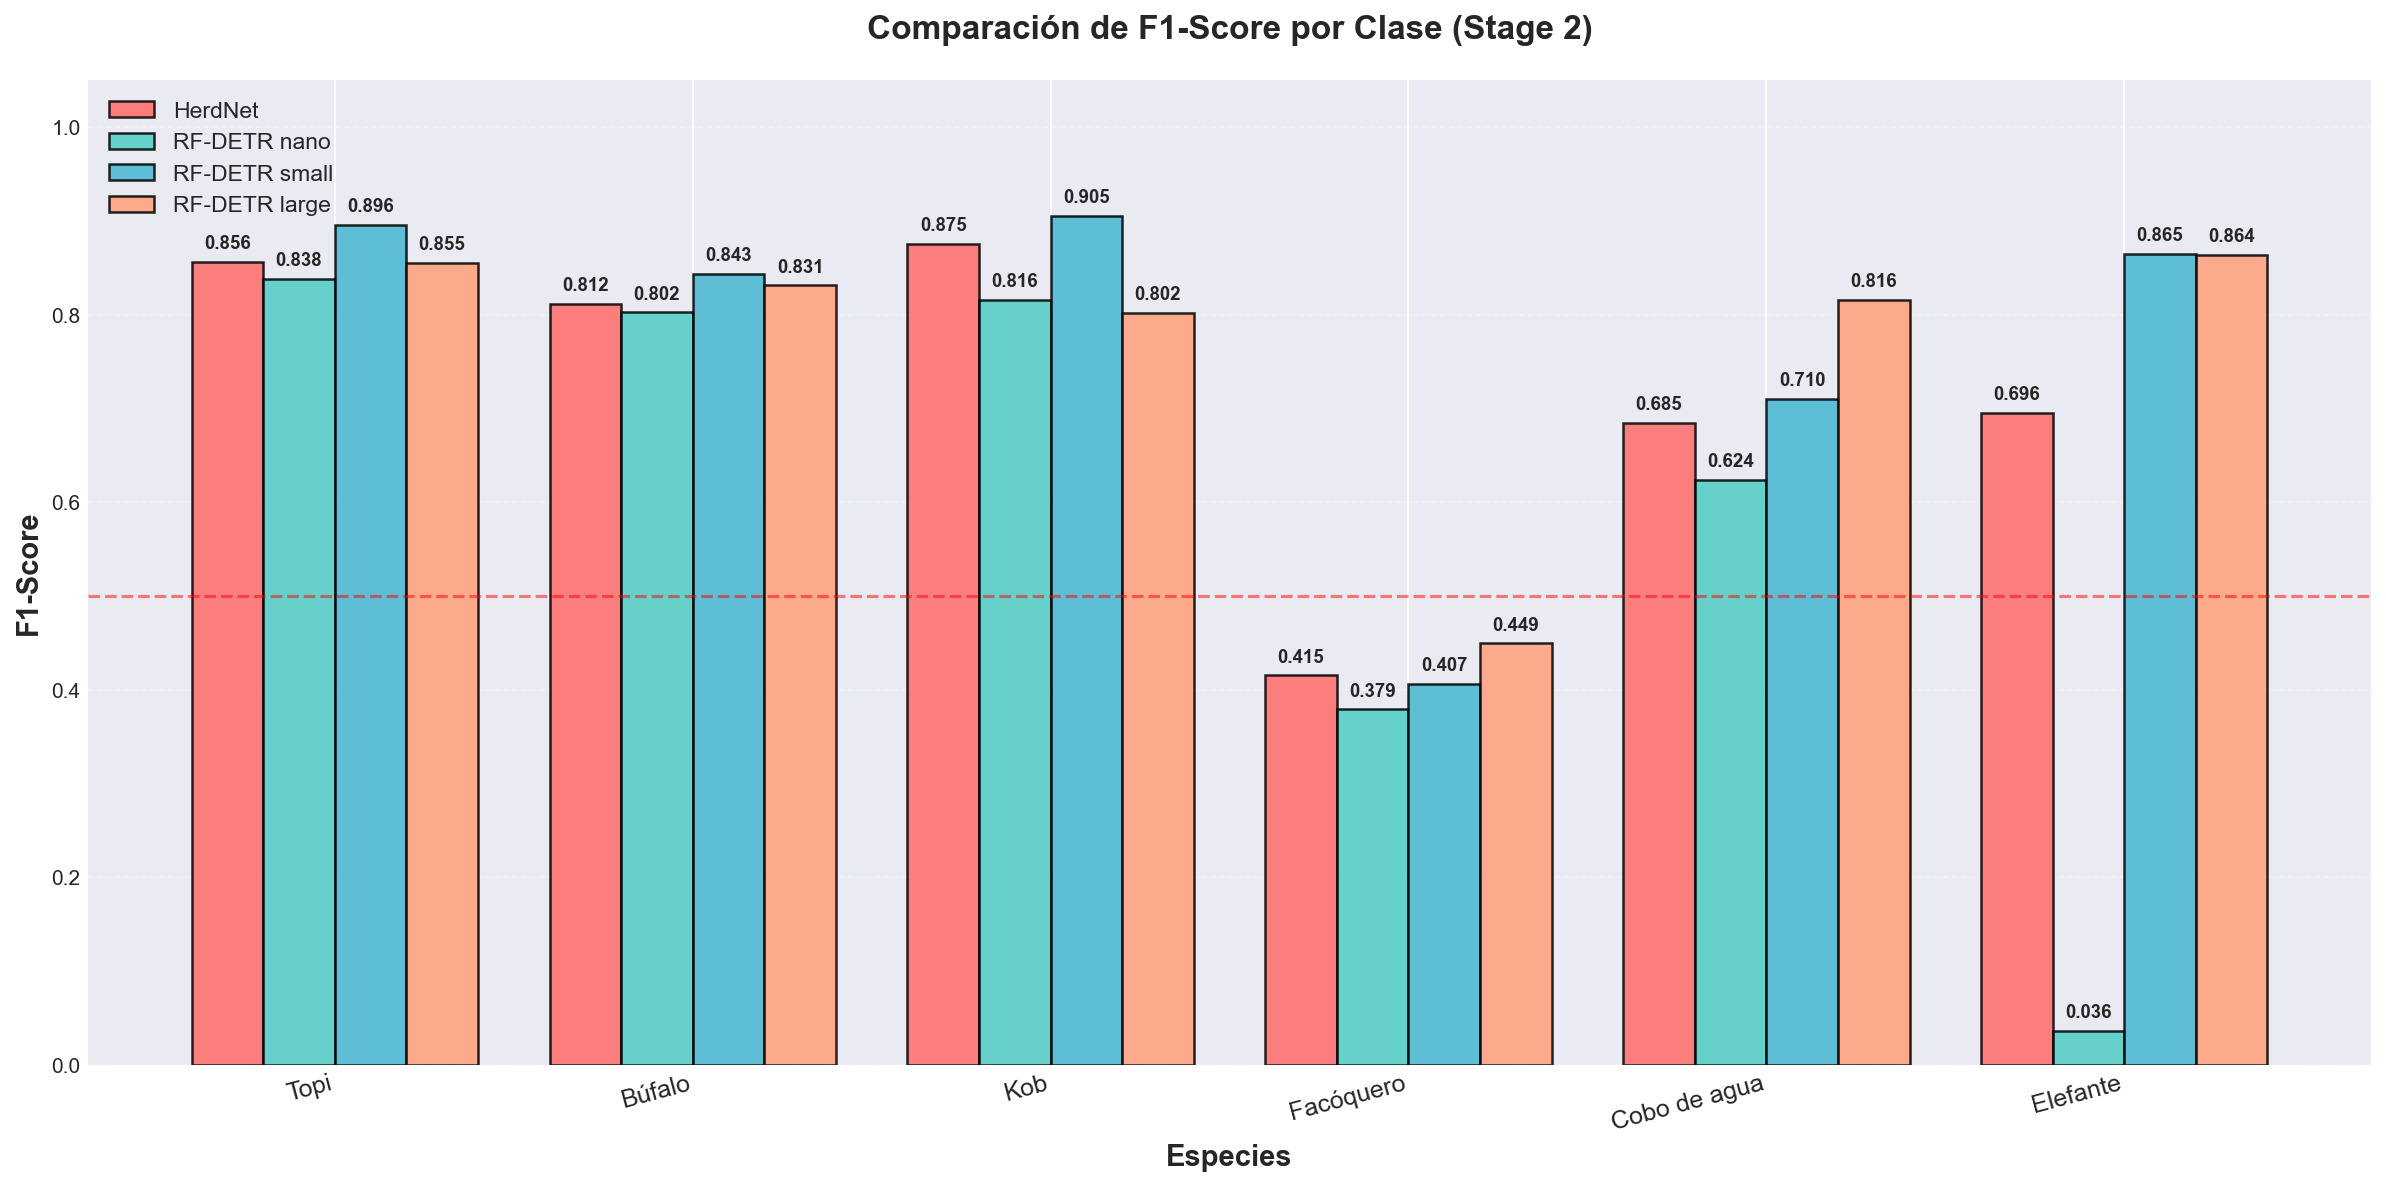
\includegraphics[width=\textwidth]{static/img/f1_score_por_clase_stage2.png}
%     \caption{F1-Score por especie para todos los modelos en Fase 2.}
%     \label{fig:f1_per_class}
% \end{figure*}
%
% Los resultados más destacados se observan en las dos especies minoritarias del dataset:
%
% \textbf{Cobo de agua:} RF-DETR large alcanzó un F1-Score de \textbf{0.816}, representando una mejora del \textbf{19.1\%} sobre HerdNet (0.685). Esta mejora se atribuye a un recall excepcional de 86.1\% y una precisión de 77.5\%, indicando que el modelo captura exitosamente la mayoría de los individuos de esta especie extremadamente subrepresentada (241 individuos en total, apenas el 2.4\% del dataset).
%
% \textbf{Facóquero:} Aunque la mejora fue más modesta, RF-DETR large alcanzó un F1-Score de 0.449 versus 0.415 de HerdNet (mejora del 8.2\%). Sin embargo, la precisión mejoró significativamente (0.484 vs 0.388), reduciendo los falsos positivos en un 24.7\%.
%
% Para especies mayoritarias como Elefante y Kob, el rendimiento tuvo mejoras incrementales de RF-DETR. Lo que indica que no se sacrifica el rendimiento en clases bien representadas mientras se mejora sustancialmente la detección de especies minoritarias, un equilibrio crítico para aplicaciones reales de monitoreo multiespecie.

\subsection{Per-Species Analysis and Minority Classes}

Figure \ref{fig:f1_per_class} presents the F1-Score disaggregated by species, revealing differentiated performance patterns that validate one of the central hypotheses of this work: Transformers improve discrimination in minority species.

\begin{figure*}[t]
    \centering
    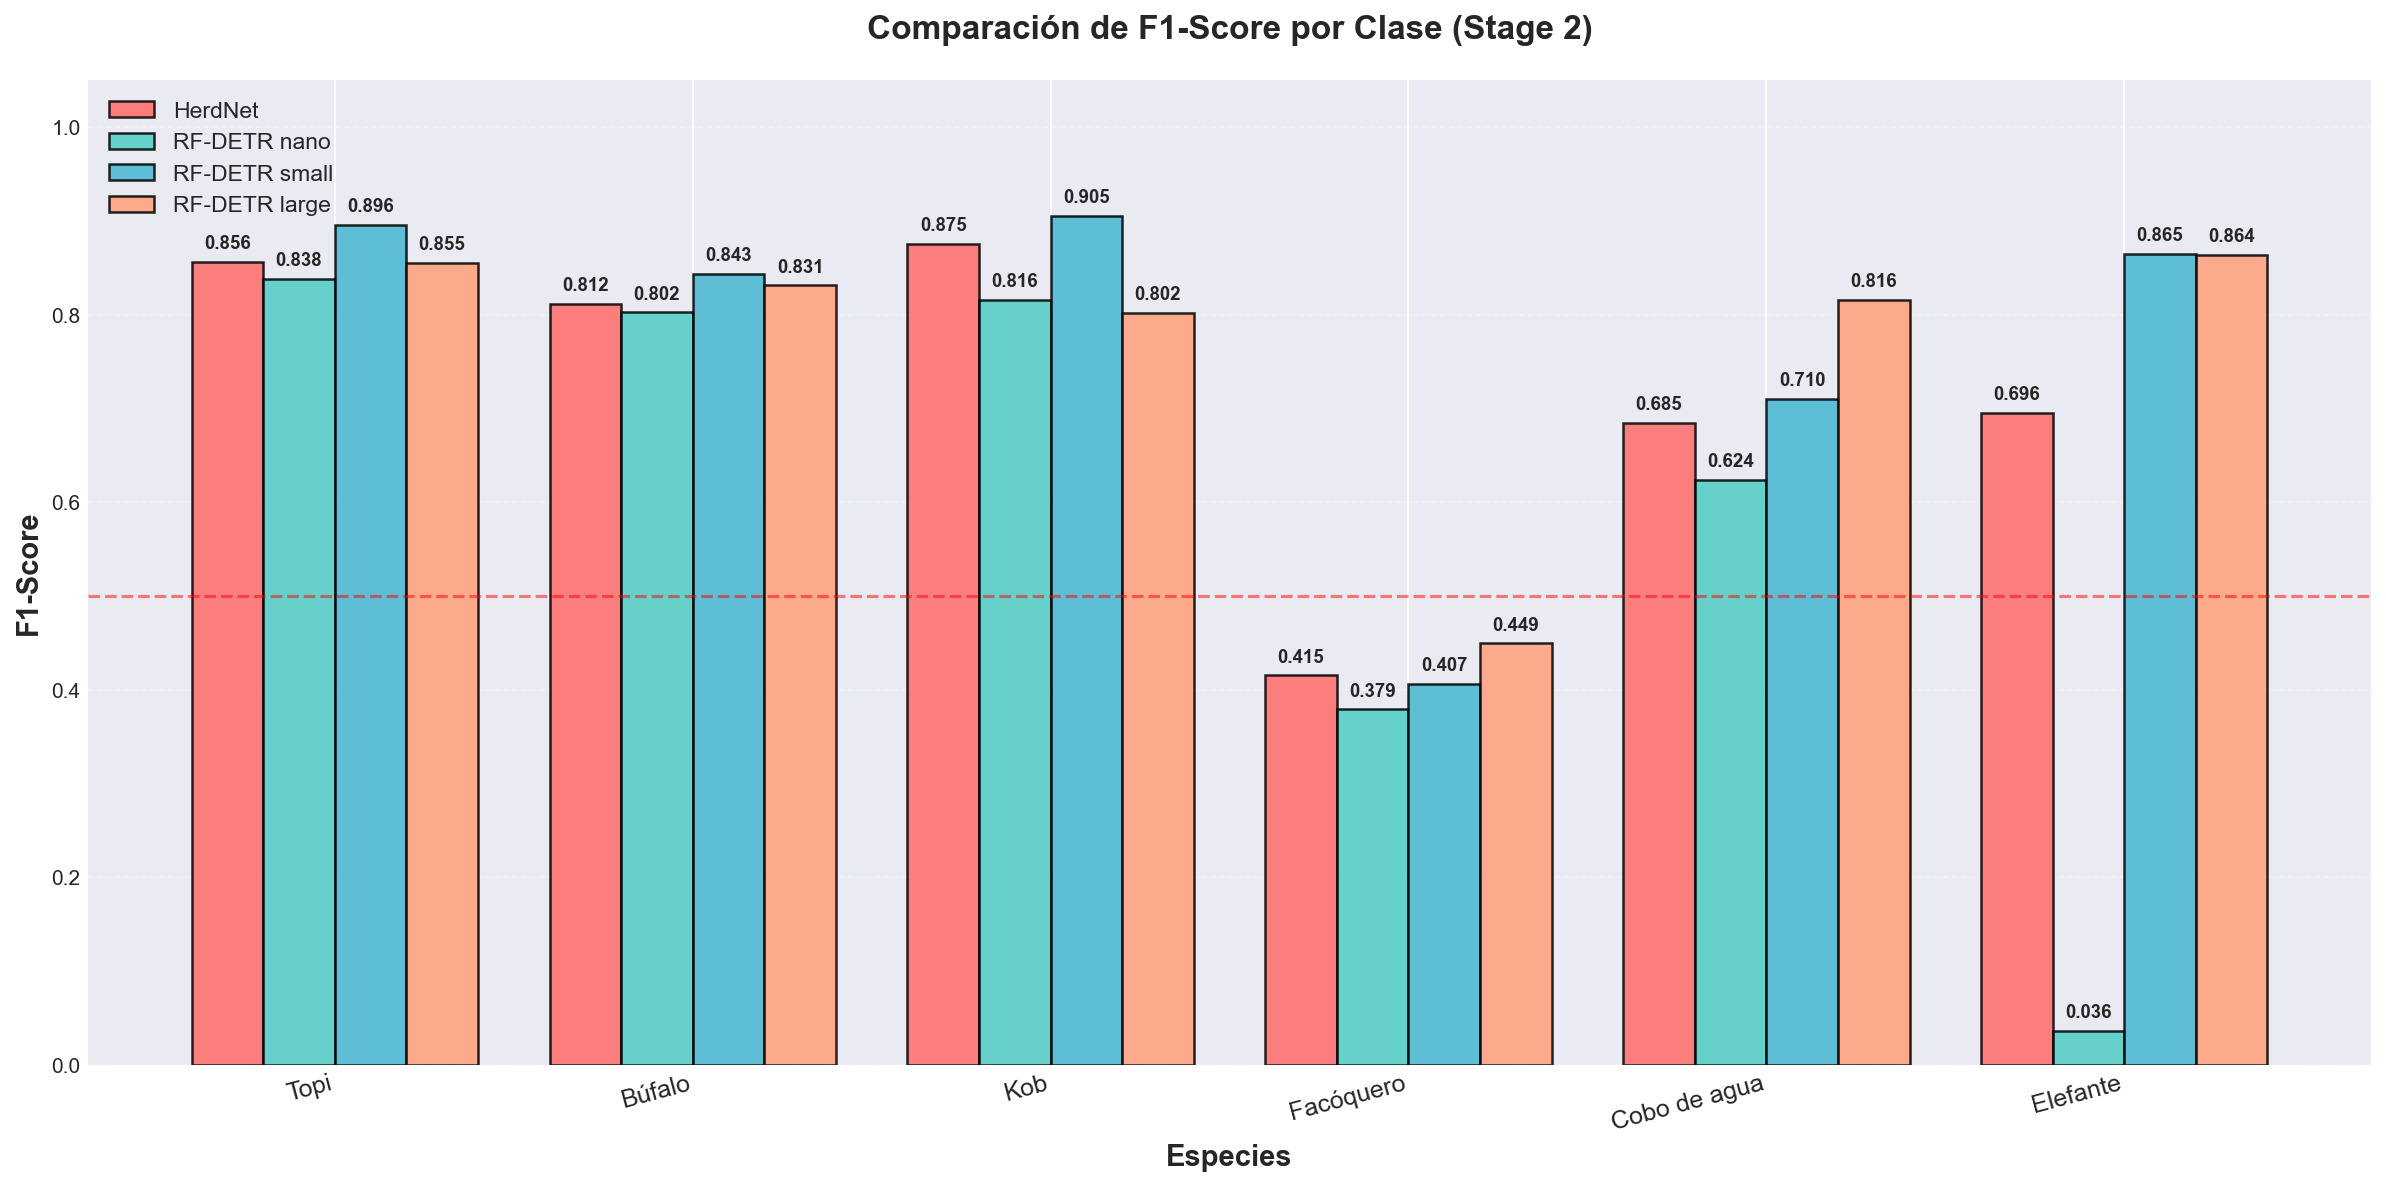
\includegraphics[width=\textwidth]{static/img/f1_score_por_clase_stage2.png}
    \caption{F1-Score per species for all models in Phase 2.}
    \label{fig:f1_per_class}
\end{figure*}

The most outstanding results are observed in the two minority species of the dataset:

\textbf{Waterbuck:} RF-DETR large achieved an F1-Score of \textbf{0.816}, representing an improvement of \textbf{19.1\%} over HerdNet (0.685). This improvement is attributed to an exceptional recall of 86.1\% and a precision of 77.5\%, indicating that the model successfully captures most individuals of this extremely underrepresented species (241 individuals in total, barely 2.4\% of the dataset).

\textbf{Warthog:} Although the improvement was more modest, RF-DETR large achieved an F1-Score of 0.449 versus 0.415 for HerdNet (8.2\% improvement). However, precision improved significantly (0.484 vs 0.388), reducing false positives by 24.7\%.

For majority species such as Elephant and Kob, performance had incremental improvements from RF-DETR. This indicates that performance on well-represented classes is not sacrificed while substantially improving detection of minority species, a critical balance for real multi-species monitoring applications.

% \subsection{Impacto del Hard Negative Mining}
%
% Como se observa en la Tabla \ref{tab:overall_metrics}, la estrategia de dos fases con HNM fue fundamental para alcanzar el rendimiento final reportado. La comparación entre Fase 1 y Fase 2 revela mejoras diferenciadas según la arquitectura, reflejando distintos niveles de susceptibilidad a la generación de falsos positivos durante el entrenamiento inicial.
%
% \textbf{RF-DETR small} mostró el impacto más significativo del HNM, con un incremento en precisión de 0.26 a 0.94 (mejora relativa del \textbf{258.9\%}), lo que indica que el modelo sin refinamiento presentaba una alta tasa de falsos positivos en patrones ambiguos. El F1-Score pasó de 0.41 a 0.90 (mejora del \textbf{119.9\%}), transformándolo de un modelo con rendimiento limitado a la mejor solución del estudio. Este comportamiento sugiere que la arquitectura small, con su mayor capacidad expresiva, es particularmente susceptible a generar falsos positivos en fondos complejos cuando se entrena sin ejemplos negativos difíciles.
%
% En contraste, \textbf{HerdNet} y \textbf{RF-DETR large} mostraron mejoras más moderadas pero consistentes. HerdNet incrementó su precisión en +33.7\% (de 0.62 a 0.82) y su F1-Score en +15.6\% (de 0.72 a 0.83), mientras que RF-DETR large mejoró +45.0\% en precisión (de 0.61 a 0.89) y +20.3\% en F1-Score (de 0.74 a 0.89). Estas mejoras más moderadas indican que ambas arquitecturas poseían cierta robustez intrínseca contra falsos positivos desde la Fase 1, requiriendo un refinamiento menos agresivo. \textbf{RF-DETR nano}, por su parte, mejoró su precisión en +62.5\% (de 0.50 a 0.82), aunque su F1-Score final (0.72) permaneció por debajo del baseline, confirmando las limitaciones arquitectónicas de la variante más compacta.
%
% La incorporación sistemática de estos ejemplos difíciles en la Fase 2 permitió a los modelos desarrollar representaciones más discriminativas, aprendiendo a distinguir características texturales y contextuales sutiles que separan animales reales de elementos de background visualmente similares.

\subsection{Impact of Hard Negative Mining}

As observed in Table \ref{tab:overall_metrics}, the two-phase strategy with HNM was fundamental to achieve the final reported performance. The comparison between Phase 1 and Phase 2 reveals differentiated improvements according to architecture, reflecting different levels of susceptibility to false positive generation during initial training.

\textbf{RF-DETR small} showed the most significant impact from HNM, with an increase in precision from 0.26 to 0.94 (relative improvement of \textbf{258.9\%}), indicating that the model without refinement exhibited a high rate of false positives on ambiguous patterns. The F1-Score went from 0.41 to 0.90 (improvement of \textbf{119.9\%}), transforming it from a model with limited performance to the best solution of the study. This behavior suggests that the small architecture, with its greater expressive capacity, is particularly susceptible to generating false positives on complex backgrounds when trained without hard negative examples.

In contrast, \textbf{HerdNet} and \textbf{RF-DETR large} showed more moderate but consistent improvements. HerdNet increased its precision by +33.7\% (from 0.62 to 0.82) and its F1-Score by +15.6\% (from 0.72 to 0.83), while RF-DETR large improved +45.0\% in precision (from 0.61 to 0.89) and +20.3\% in F1-Score (from 0.74 to 0.89). These more moderate improvements indicate that both architectures possessed certain intrinsic robustness against false positives from Phase 1, requiring less aggressive refinement. \textbf{RF-DETR nano}, for its part, improved its precision by +62.5\% (from 0.50 to 0.82), although its final F1-Score (0.72) remained below the baseline, confirming the architectural limitations of the most compact variant.

The systematic incorporation of these hard examples in Phase 2 allowed the models to develop more discriminative representations, learning to distinguish subtle textural and contextual features that separate real animals from visually similar background elements.

% \subsection{Eficiencia Computacional}
%
% La Figura \ref{fig:inference_times} presenta la distribución de latencias de inferencia por imagen medidas en el conjunto de prueba utilizando una GPU NVIDIA A100 (80GB VRAM). Los diagramas de caja revelan tanto la tendencia central como la variabilidad de los tiempos de procesamiento para cada modelo.
%
% \begin{figure}[ht]
%     \centering
%     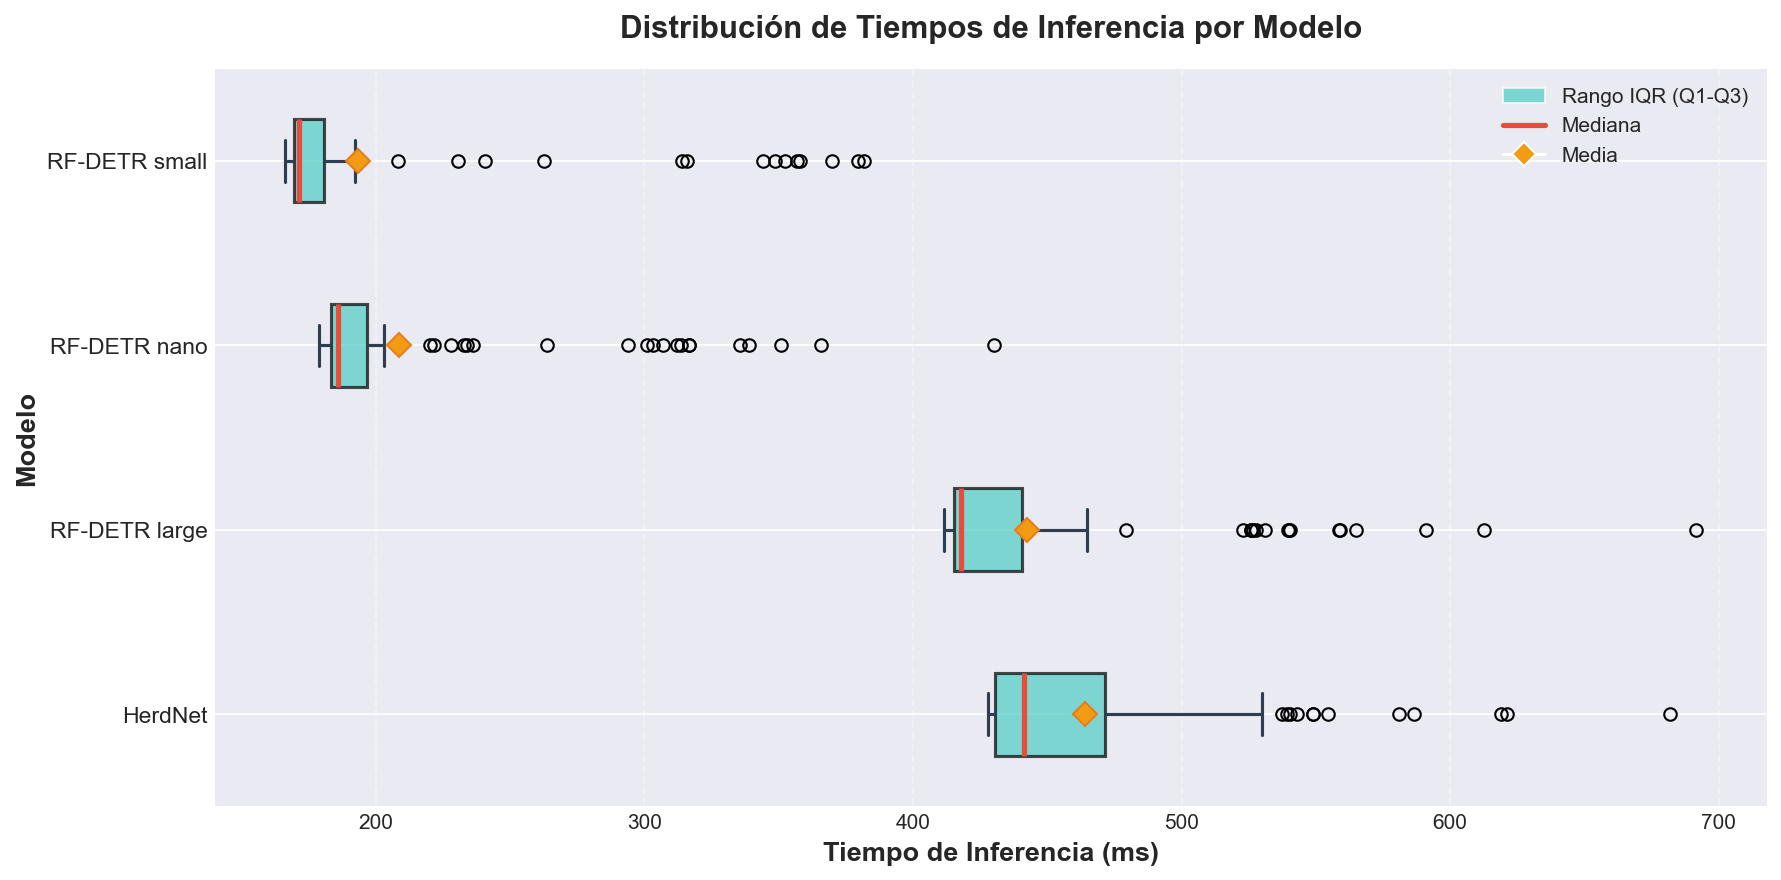
\includegraphics[width=\columnwidth]{static/img/inference_times_boxplot.png}
%     \caption{Distribución de tiempos de inferencia por modelo en conjunto de prueba. La línea roja indica la mediana y el rombo naranja la media.}
%     \label{fig:inference_times}
% \end{figure}
%
% RF-DETR small representa el modelo más eficiente, con una mediana de 171.49 ms y una media de 193.39 ms por imagen, superando incluso a RF-DETR nano (mediana: 186.16 ms, media: 208.53 ms).
%
% HerdNet y RF-DETR large presentan latencias comparables, con medianas de 441.27 ms y 417.88 ms respectivamente, siendo aproximadamente 2.4× más lentos que RF-DETR small. Sin embargo, ambos modelos exhiben mayor variabilidad temporal, como evidencian los outliers presentes en la figura, sugiriendo dependencia en la complejidad de las escenas procesadas.
%
% Para aplicaciones de monitoreo de fauna donde tanto la precisión como el throughput son críticos, RF-DETR small representa la opción óptima al combinar el mejor F1-Score con la menor latencia y mayor consistencia temporal.

\subsection{Computational Efficiency}

Figure \ref{fig:inference_times} presents the distribution of inference latencies per image measured on the test set using an NVIDIA A100 GPU (80GB VRAM). The box plots reveal both the central tendency and variability of processing times for each model.

\begin{figure}[ht]
    \centering
    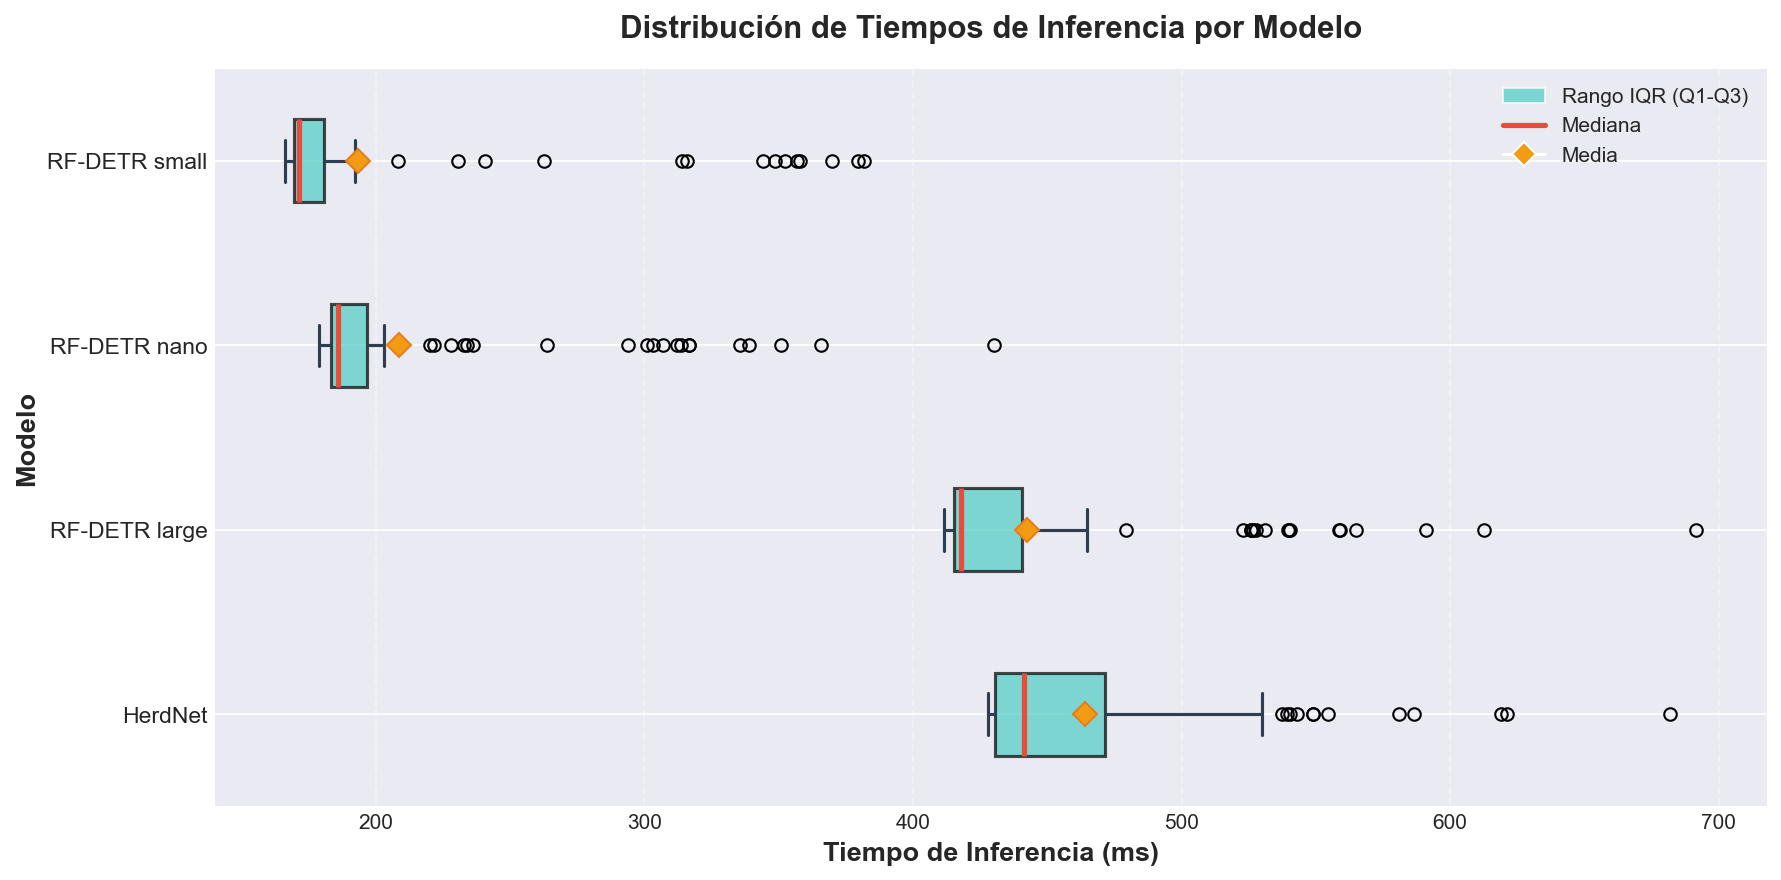
\includegraphics[width=\columnwidth]{static/img/inference_times_boxplot.png}
    \caption{Distribution of inference times per model on the test set. The red line indicates the median and the orange diamond the mean.}
    \label{fig:inference_times}
\end{figure}

RF-DETR small represents the most efficient model, with a median of 171.49 ms and a mean of 193.39 ms per image, even surpassing RF-DETR nano (median: 186.16 ms, mean: 208.53 ms).

HerdNet and RF-DETR large present comparable latencies, with medians of 441.27 ms and 417.88 ms respectively, being approximately 2.4× slower than RF-DETR small. However, both models exhibit greater temporal variability, as evidenced by the outliers present in the figure, suggesting dependence on the complexity of the processed scenes.

For wildlife monitoring applications where both precision and throughput are critical, RF-DETR small represents the optimal option by combining the best F1-Score with the lowest latency and greatest temporal consistency.

% \subsection{Análisis de Matrices de Confusión sobre las detecciones}
%
% La Figura \ref{fig:confusion_matrix} presenta la matriz sobre las detecciones para RF-DETR small, el modelo de mejor desempeño.
%
% \begin{figure}[ht]
%     \centering
%     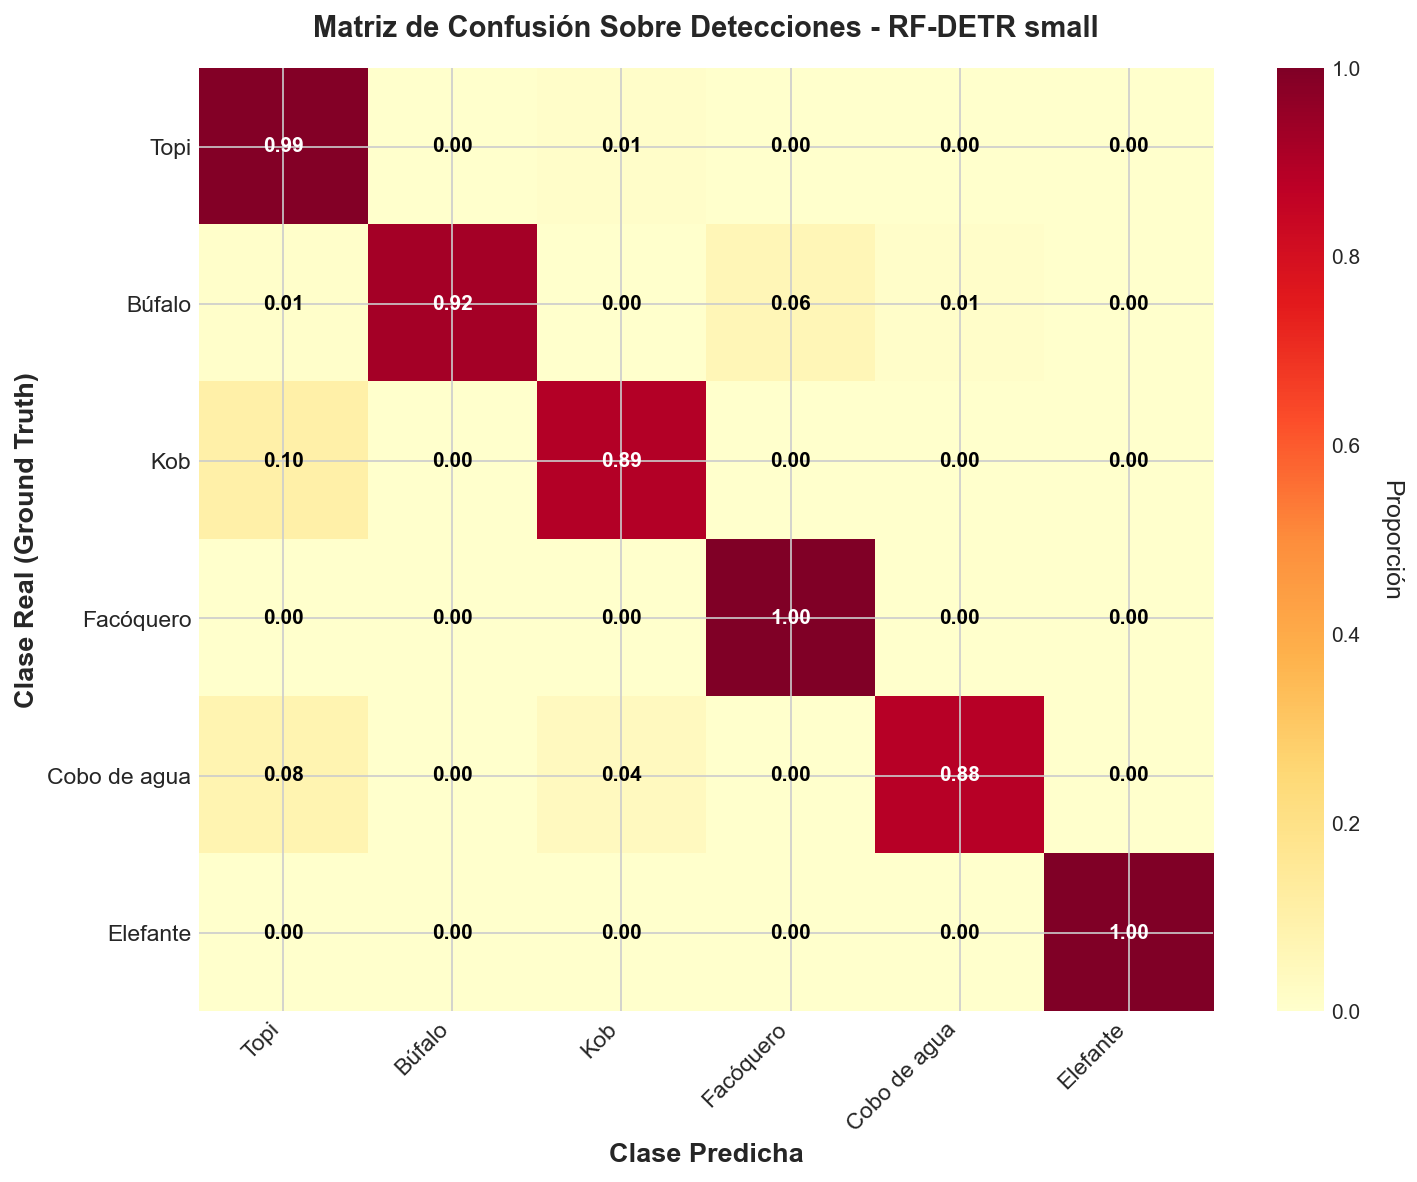
\includegraphics[width=\columnwidth]{static/img/confusion_matrix_rf-detr_small_stage2.png}
%     \caption{Matriz de confusión sobre las detecciones para RF-DETR small (Fase 2).}
%     \label{fig:confusion_matrix}
% \end{figure}
%
% El análisis de la diagonal principal revela una alta eficacia en la clasificación correcta para la mayoría de las especies: Topi (99\%), Búfalo (92\%), Kob (89\%) y Cobo de agua (88\%), destacando un desempeño perfecto (100\%) en las clases Facóquero y Elefante.
%
% Los patrones de confusión interespecífica más relevantes son:
%
% \begin{itemize}
%     \item \textbf{Kob $\rightarrow$ Topi (10\%):} Representa la confusión más significativa del modelo. Es un error unidireccional (la inversa es despreciable), atribuible a la similitud morfológica entre estos antílopes de tamaño medio y pelaje rojizo. El modelo parece identificar mejor los rasgos distintivos del Topi (cuernos curvados y manchas oscuras en las patas) que la morfología más genérica del Kob en ciertas posturas.
%
%     \item \textbf{Cobo de agua $\rightarrow$ Antílopes (12\%):} Esta especie presenta confusiones divididas: un 8\% es clasificado erróneamente como Topi y un 4\% como Kob. Estas confusiones ocurren típicamente cuando el animal está parcialmente ocluido o en ángulos cenitales estrictos donde sus cuernos característicos en forma de lira no son visibles, llevando al modelo a asignarlo a las clases de antílopes mayoritarias.
%
%     \item \textbf{Búfalo $\rightarrow$ Facóquero (6\%):} Se observa una confusión del 6\% de Búfalos clasificados como Facóqueros. Este error, aunque contraintuitivo por la diferencia de tamaño real, puede explicarse por la similitud en la coloración oscura y la textura de la piel en individuos juveniles o en tomas donde la escala relativa es ambigua debido a la altitud de vuelo.
% \end{itemize}

\subsection{Confusion Matrix Analysis on Detections}

Figure \ref{fig:confusion_matrix} presents the confusion matrix on detections for RF-DETR small, the best performing model.

\begin{figure}[ht]
    \centering
    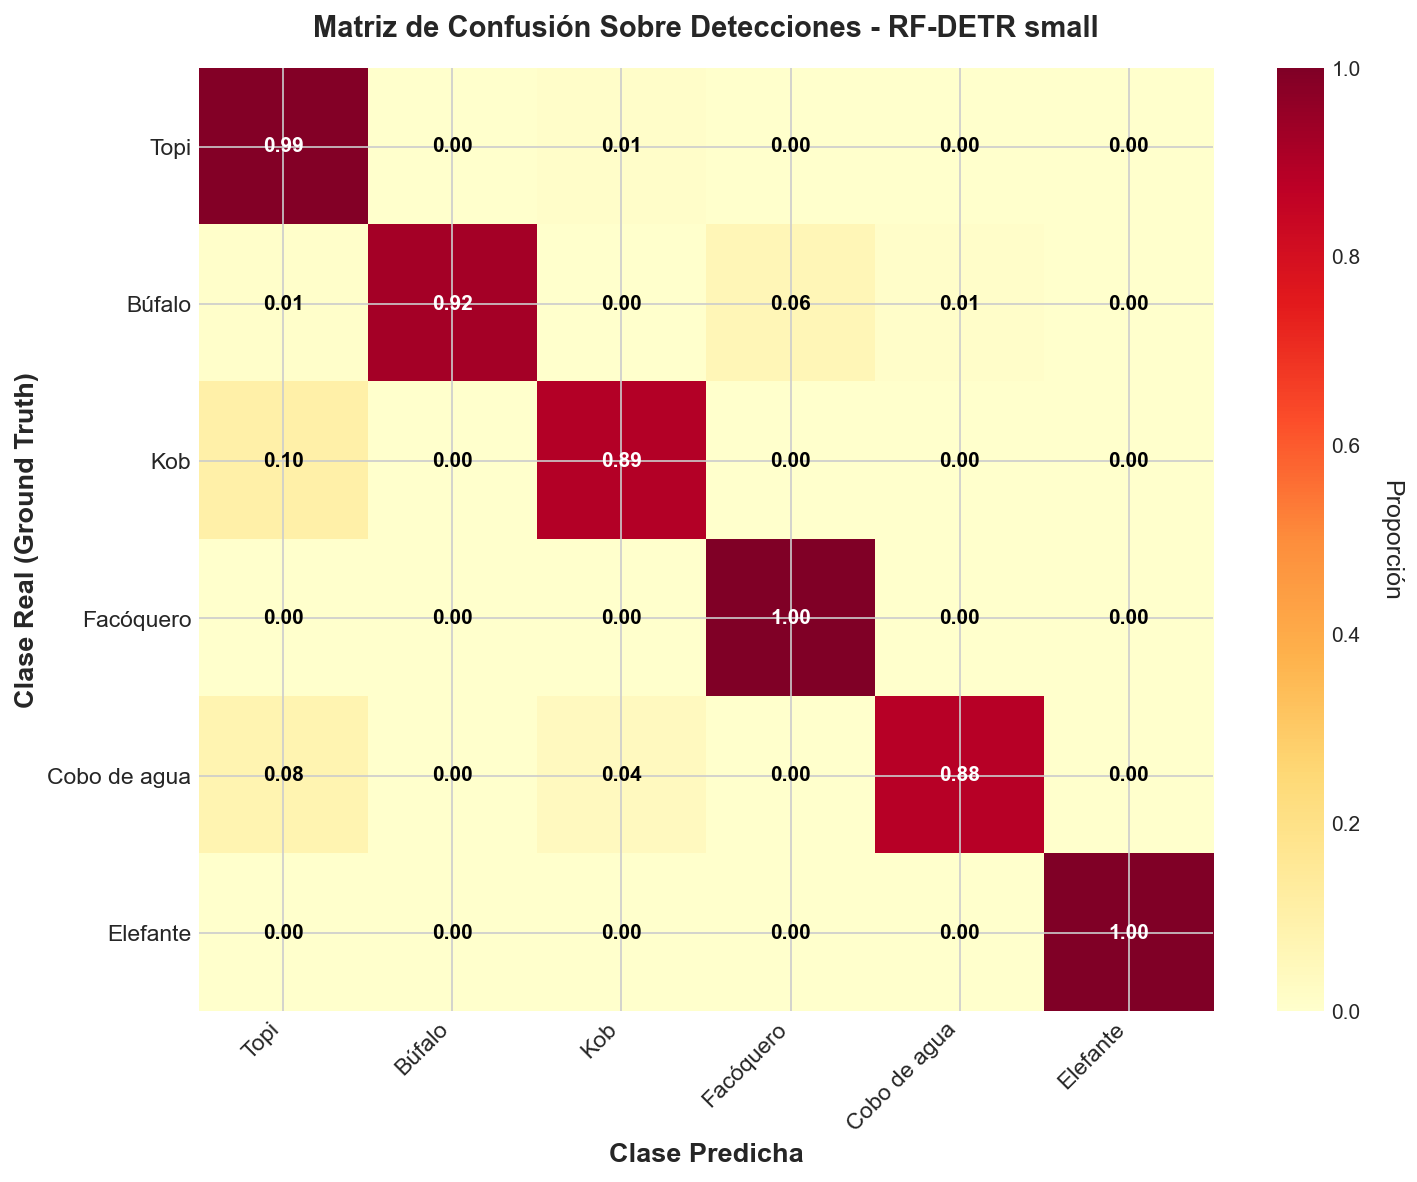
\includegraphics[width=\columnwidth]{static/img/confusion_matrix_rf-detr_small_stage2.png}
    \caption{Confusion matrix on detections for RF-DETR small (Phase 2).}
    \label{fig:confusion_matrix}
\end{figure}

Analysis of the main diagonal reveals high efficacy in correct classification for most species: Topi (99\%), Buffalo (92\%), Kob (89\%), and Waterbuck (88\%), with perfect performance (100\%) standing out in the Warthog and Elephant classes.

The most relevant interspecific confusion patterns are:

\begin{itemize}
    \item \textbf{Kob $\rightarrow$ Topi (10\%):} Represents the model's most significant confusion. It is a unidirectional error (the inverse is negligible), attributable to the morphological similarity between these medium-sized antelopes with reddish fur. The model seems to better identify the distinctive features of Topi (curved horns and dark spots on the legs) than the more generic morphology of Kob in certain postures.

    \item \textbf{Waterbuck $\rightarrow$ Antelopes (12\%):} This species presents divided confusions: 8\% is erroneously classified as Topi and 4\% as Kob. These confusions typically occur when the animal is partially occluded or at strict zenith angles where its characteristic lyre-shaped horns are not visible, leading the model to assign it to the majority antelope classes.

    \item \textbf{Buffalo $\rightarrow$ Warthog (6\%):} A confusion of 6\% of Buffalos classified as Warthogs is observed. This error, although counterintuitive due to the difference in actual size, can be explained by the similarity in dark coloration and skin texture in juvenile individuals or in shots where the relative scale is ambiguous due to flight altitude.
\end{itemize}

% \subsubsection{Interpretación de la Clasificación Perfecta}
% Es notable que especies como el \textbf{Facóquero} y el \textbf{Elefante} alcancen un 100\% en la diagonal de la matriz. Sin embargo, este resultado debe interpretarse con rigor técnico:
%
% \begin{itemize}
%     \item \textbf{Pureza vs. Exhaustividad:} El 100\% en la matriz indica una \textbf{precisión de clasificación condicional} perfecta: de todos los Facóqueros que el modelo logró detectar, ninguno fue confundido con otra especie.
%     \item \textbf{Discrepancia con el Recall:} Este valor no contradice el bajo \textit{Recall} de detección reportado anteriormente para el Facóquero (33.78\%). Significa que el modelo omite muchos individuos (falsos negativos de localización), pero cuando detecta uno, su clasificación semántica es impecable. Esto valida la efectividad del \textit{HNP} para limpiar la frontera de decisión entre la clase Facóquero y el fondo, aunque la arquitectura aún lucha por recuperar instancias difíciles.
% \end{itemize}
%
% En conclusión, las confusiones se concentran en el clúster de antílopes (Kob-Topi-Cobo), mientras que las especies con morfologías más distintivas (Elefante, Facóquero, Búfalo) presentan una separabilidad semántica robusta.

\subsubsection{Interpretation of Perfect Classification}
It is notable that species such as \textbf{Warthog} and \textbf{Elephant} achieve 100\% on the matrix diagonal. However, this result must be interpreted with technical rigor:

\begin{itemize}
    \item \textbf{Purity vs. Exhaustiveness:} The 100\% in the matrix indicates perfect \textbf{conditional classification precision}: of all the Warthogs that the model managed to detect, none were confused with another species.
    \item \textbf{Discrepancy with Recall:} This value does not contradict the low detection \textit{Recall} previously reported for Warthog (33.78\%). It means that the model omits many individuals (localization false negatives), but when it detects one, its semantic classification is impeccable. This validates the effectiveness of \textit{HNM} to clean the decision boundary between the Warthog class and the background, although the architecture still struggles to recover difficult instances.
\end{itemize}

In conclusion, confusions are concentrated in the antelope cluster (Kob-Topi-Waterbuck), while species with more distinctive morphologies (Elephant, Warthog, Buffalo) present robust semantic separability.

% \subsection{Evaluación Cualitativa en Especies Minoritarias}
%
% Se realizó una evaluación cualitativa enfocada en especies minoritarias bajo condiciones críticas de detección. Las Figuras \ref{fig:qualitative_elephant} y \ref{fig:qualitative_warthog} comparan las predicciones de los modelos contra Ground Truth en dos escenarios representativos.
%
% \begin{figure*}[t]
%     \centering
%     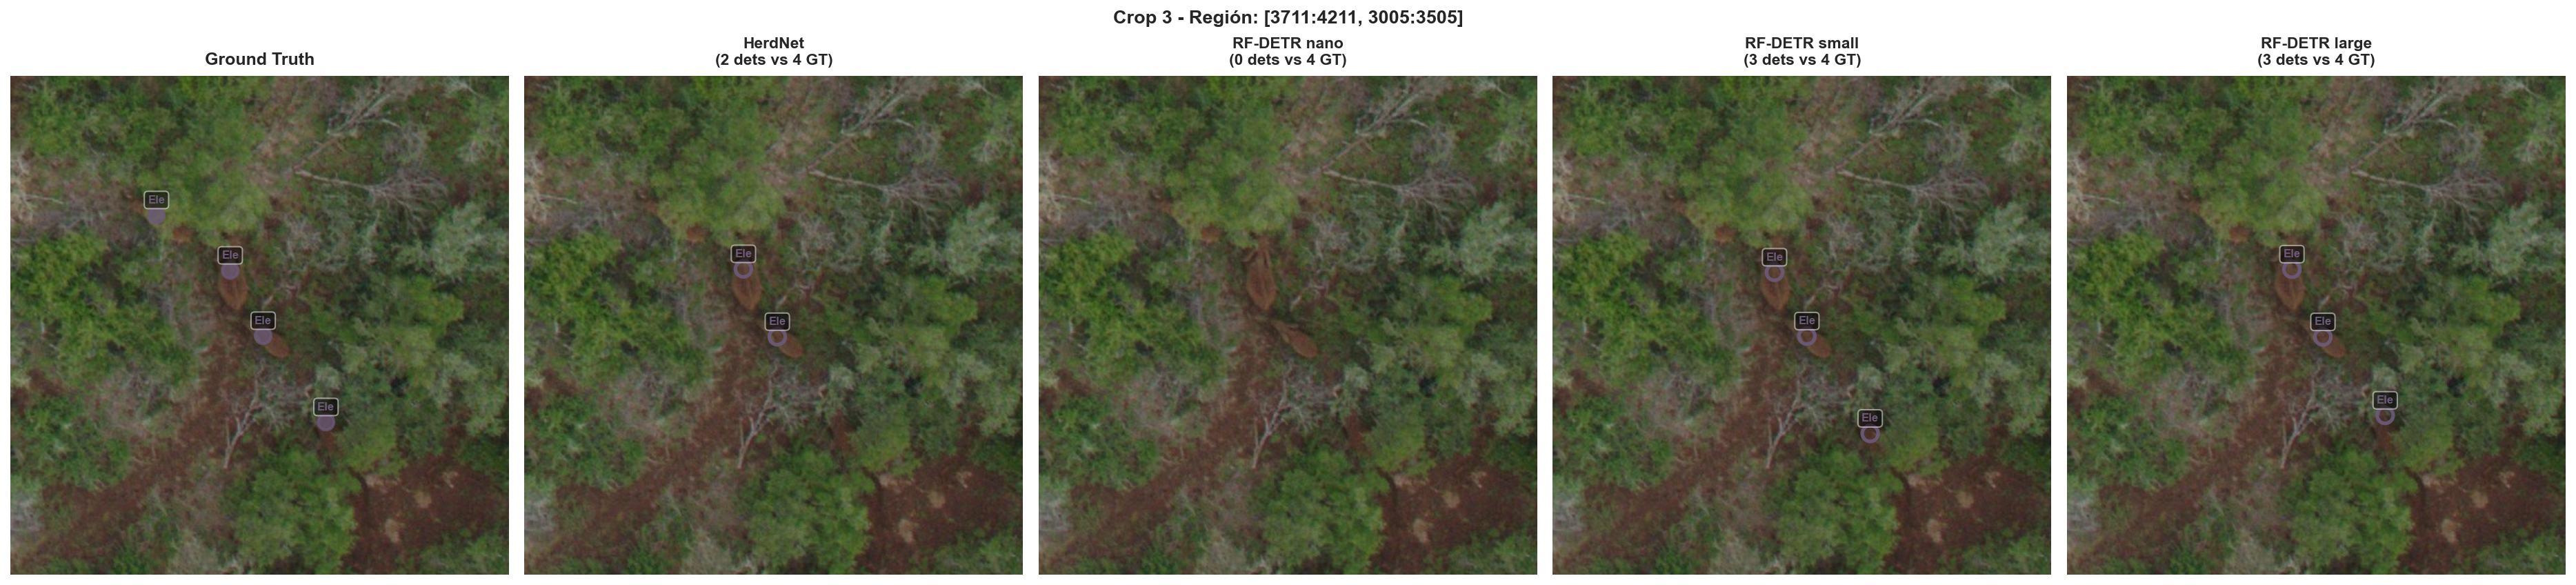
\includegraphics[width=\textwidth]{static/img/comparison_panel_elefante_crop3_stage2.png}
%     \caption{Comparación cualitativa de detecciones en escenario con oclusión severa - Elefantes. Se observan 4 elefantes parcialmente ocultos por vegetación densa.}
%     \label{fig:qualitative_elephant}
% \end{figure*}
%
% \begin{figure*}[t]
%     \centering
%     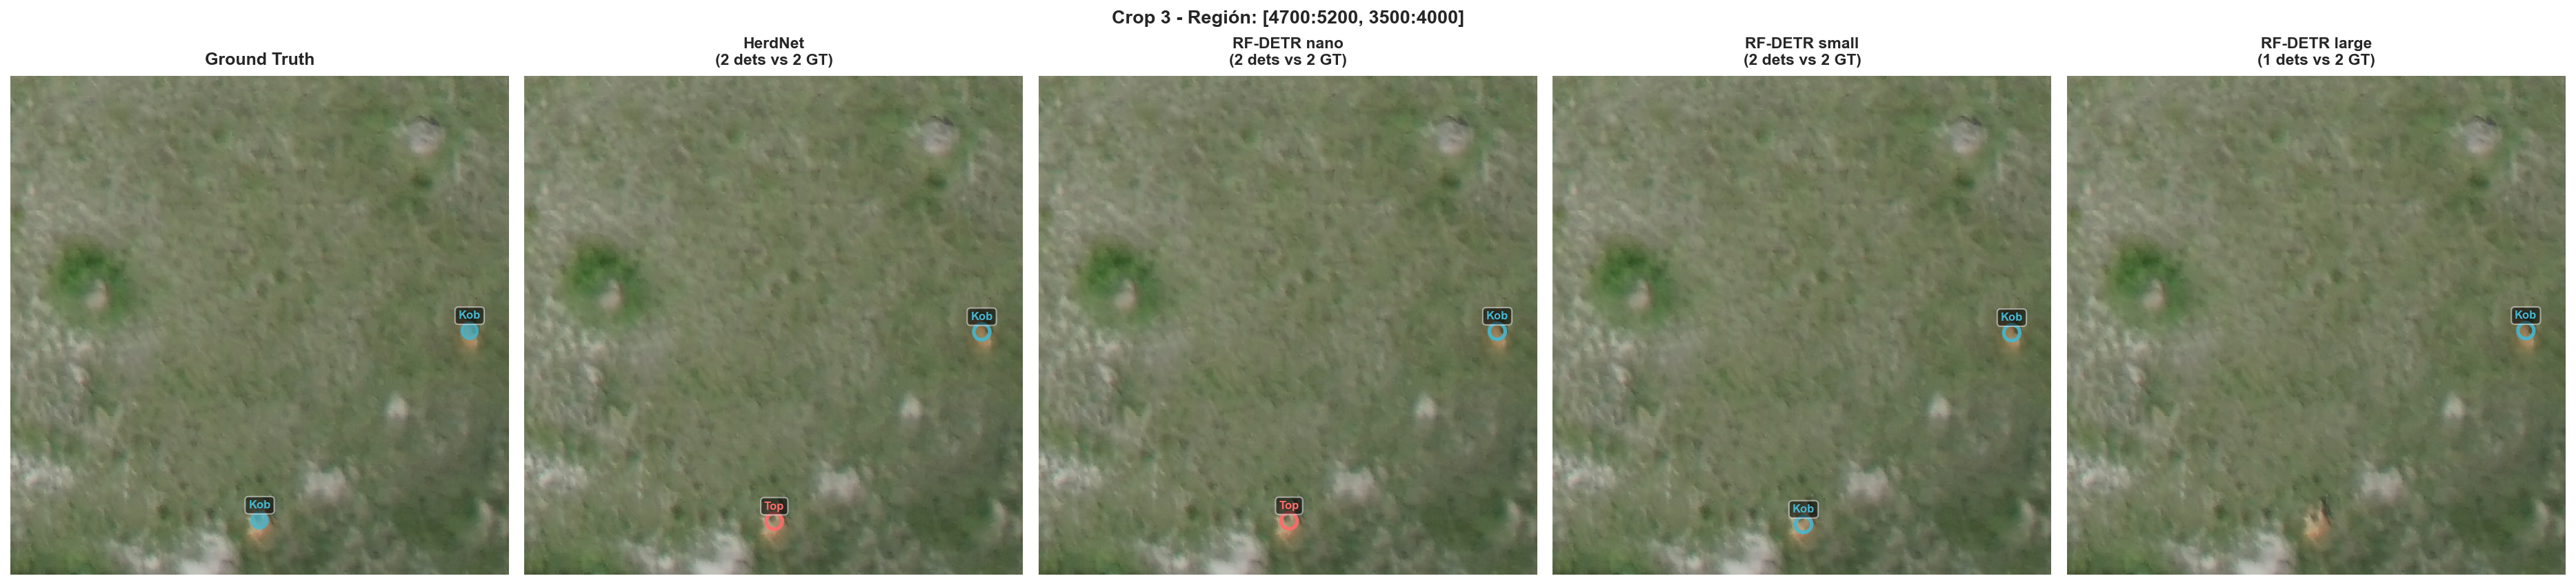
\includegraphics[width=\textwidth]{static/img/comparison_panel_facoquero_crop3_stage2.png}
%     \caption{Comparación cualitativa de detecciones en especies minoritarias - Facóquero. Se muestran 2 individuos aislados en terreno de vegetación dispersa.}
%     \label{fig:qualitative_warthog}
% \end{figure*}

\subsection{Qualitative Evaluation on Minority Species}

A qualitative evaluation focused on minority species under critical detection conditions was performed. Figures \ref{fig:qualitative_elephant} and \ref{fig:qualitative_warthog} compare model predictions against Ground Truth in two representative scenarios.

\begin{figure*}[t]
    \centering
    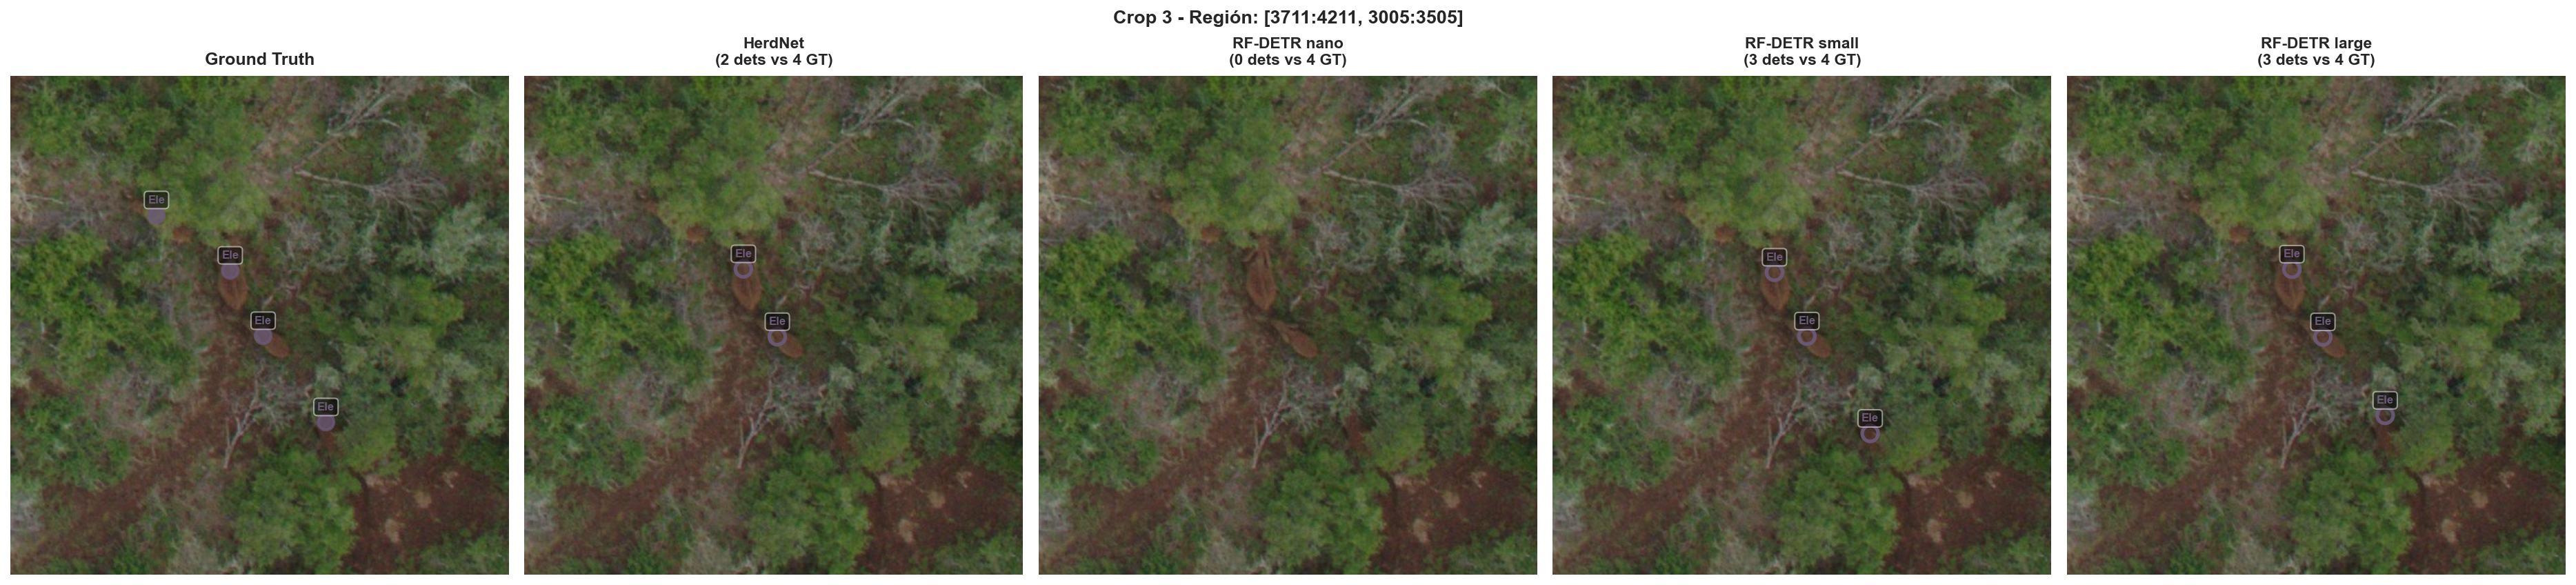
\includegraphics[width=\textwidth]{static/img/comparison_panel_elefante_crop3_stage2.png}
    \caption{Qualitative comparison of detections in a scenario with severe occlusion - Elephants. Four elephants partially hidden by dense vegetation are observed.}
    \label{fig:qualitative_elephant}
\end{figure*}

\begin{figure*}[t]
    \centering
    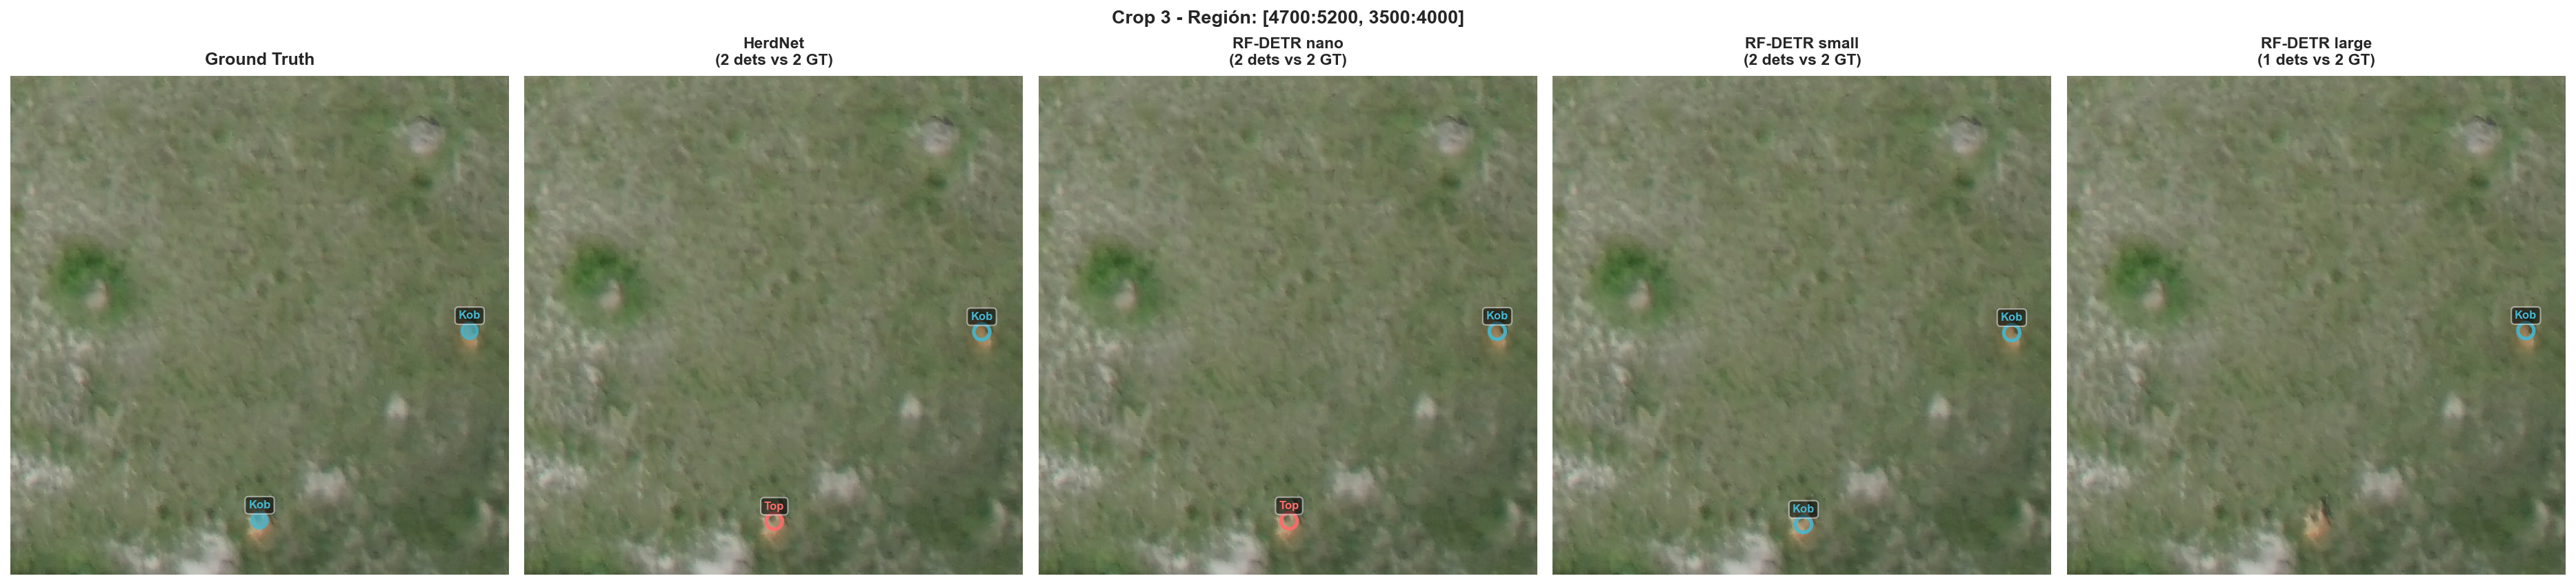
\includegraphics[width=\textwidth]{static/img/comparison_panel_facoquero_crop3_stage2.png}
    \caption{Qualitative comparison of detections on minority species - Warthog. Two isolated individuals are shown in terrain with dispersed vegetation.}
    \label{fig:qualitative_warthog}
\end{figure*}


% \subsubsection{Caso 1: Oclusión Severa en Elefantes}
%
% La Figura \ref{fig:qualitative_elephant} ilustra cuatro elefantes parcialmente ocultos por vegetación densa. Los resultados de detección son:
%
% \begin{itemize}
%     \item \textbf{HerdNet:} 2/4 detecciones (50\%). Falla en individuos con características distintivas ocultas (trompa, orejas), reflejando limitaciones del backbone ResNet-50 para capturar contexto global.
%     \item \textbf{RF-DETR small y large:} 3/4 detecciones (75\%). Mejora del +50\% sobre HerdNet, detectando exitosamente individuos con hasta 50\% de oclusión.
% \end{itemize}
%
% \textbf{Hallazgo clave:} La oclusión representa un límite fundamental para todos los modelos, incluyendo arquitecturas Transformer. Aunque RF-DETR mejora significativamente sobre HerdNet, existe un umbral de oclusión que ningún modelo supera, y \textbf{RF-DETR nano} carece de la capacidad mínima necesaria para escenarios complejos.

\subsubsection{Case 1: Severe Occlusion in Elephants}

Figure \ref{fig:qualitative_elephant} illustrates four elephants partially hidden by dense vegetation. The detection results are:

\begin{itemize}
    \item \textbf{HerdNet:} 2/4 detections (50\%). Fails on individuals with hidden distinctive features (trunk, ears), reflecting limitations of the ResNet-50 backbone to capture global context.
    \item \textbf{RF-DETR small and large:} 3/4 detections (75\%). +50\% improvement over HerdNet, successfully detecting individuals with up to 50\% occlusion.
\end{itemize}

\textbf{Key finding:} Occlusion represents a fundamental limit for all models, including Transformer architectures. Although RF-DETR significantly improves over HerdNet, there exists an occlusion threshold that no model surpasses, and \textbf{RF-DETR nano} lacks the minimum capacity necessary for complex scenarios.

% \subsubsection{Caso 2: Detección y Clasificación de Facóquero}
%
% La Figura \ref{fig:qualitative_warthog} presenta dos facóqueros en terreno abierto , revelando un patrón diferente de error: confusión en clasificación pese a detección correcta.
%
% \begin{itemize}
%     \item \textbf{HerdNet:} 2/2 detecciones pero 1/2 clasificación correcta (50\%). Detecta ambos individuos en las ubicaciones correctas pero clasifica uno erróneamente como Topi, evidenciando las limitaciones del backbone ResNet-50 para discriminar especies morfológicamente similares de tamaño medio.
%     \item \textbf{RF-DETR  small:} 2/2 detecciones y clasificación correcta (100\%). Lo que demuestra capacidad superior para discriminar Facóquero bajo condiciones de buena visibilidad, validando la efectividad del refinamiento mediante HNM y los mecanismos de atención.
% \end{itemize}
%
% \textbf{Hallazgos clave:} Este caso revela dos patrones críticos: (1) Con buena visibilidad, la detección espacial es exitosa incluso para HerdNet, pero la clasificación correcta requiere capacidades discriminativas superiores que solo los Transformers proveen. (2) Para especies minoritarias morfológicamente similares a especies mayoritarias (Facóquero vs Kob), los modelos CNN tienden a clasificar hacia la clase más frecuente, mientras que RF-DETR mantiene discriminación robusta. Esto valida la clasificación perfecta (100\%) de Facóquero reportada en la matriz de confusión para RF-DETR small.

\subsubsection{Case 2: Warthog Detection and Classification}

Figure \ref{fig:qualitative_warthog} presents two warthogs in open terrain, revealing a different error pattern: classification confusion despite correct detection.

\begin{itemize}
    \item \textbf{HerdNet:} 2/2 detections but 1/2 correct classification (50\%). Detects both individuals in the correct locations but erroneously classifies one as Topi, evidencing the limitations of the ResNet-50 backbone to discriminate morphologically similar medium-sized species.
    \item \textbf{RF-DETR small:} 2/2 detections and correct classification (100\%). This demonstrates superior capability to discriminate Warthog under good visibility conditions, validating the effectiveness of refinement through HNM and attention mechanisms.
\end{itemize}

\textbf{Key findings:} This case reveals two critical patterns: (1) With good visibility, spatial detection is successful even for HerdNet, but correct classification requires superior discriminative capabilities that only Transformers provide. (2) For minority species morphologically similar to majority species (Warthog vs Kob), CNN models tend to classify toward the most frequent class, while RF-DETR maintains robust discrimination. This validates the perfect classification (100\%) of Warthog reported in the confusion matrix for RF-DETR small.
